\subsection{Brain Tumor Datenset} \label{chap:Brain-Tumor}

\subsubsection{Hirntumor} \label{chap:Hirntumor}
Hirntumoren sind abnormale Wucherungen von Zellen im Gehirn, die entweder gutartig oder bösartig sein können. Diese Tumoren können sowohl im Gehirn selbst entstehen als auch als Metastasen von anderen Krebsarten in den Kopf wandern. Die Symptome variieren je nach Tumorart, -grösse und -lokalisation und können Kopfschmerzen, Übelkeit, Sehstörungen, Krampfanfälle und kognitive Beeinträchtigungen umfassen. Aufgrund ihrer Komplexität und der sensiblen Lage im zentralen Nervensystem stellen Hirntumoren eine erhebliche Herausforderung für die medizinische Diagnostik und Behandlung dar und haben oft weitreichende Auswirkungen auf die Lebensqualität der Betroffenen. 

\todo{Quelle}

\subsubsection{Datensatz}
Der \textbf{Brain Tumor Classification (MRI)-Datensatz} \cite{bhuvaji_brain_2020} umfasst 3.260 bereinigte und augmentierte, T1-gewichtete, kontrastverstärkte MRI-Bilder zur Identifikation und Klassifikation von Hirntumoren. 

Die MRI-Bilder in der Abbildung zeigen Beispiele von Gehirnscans, die zur Klassifikation von Hirntumoren verwendet werden. Positive Fälle werden mit der Klasse 1 und negative Fälle mit der Klasse 0 gekennzeichnet. Eine genaue Beschreibung der Klassenzusammenfassung findet sich in Kapitel \ref{chap:Brain-Tumor-Partition}. In den Beispielabbildungen \ref{fig:brain-klasse0} und \ref{fig:brain-klasse1} erkennen wir, dass im Datensatz Saggital-, Frontal- und Transversalebenen des Kopfes enthalten sind.

\begin{figure}[ht]
    \centering
    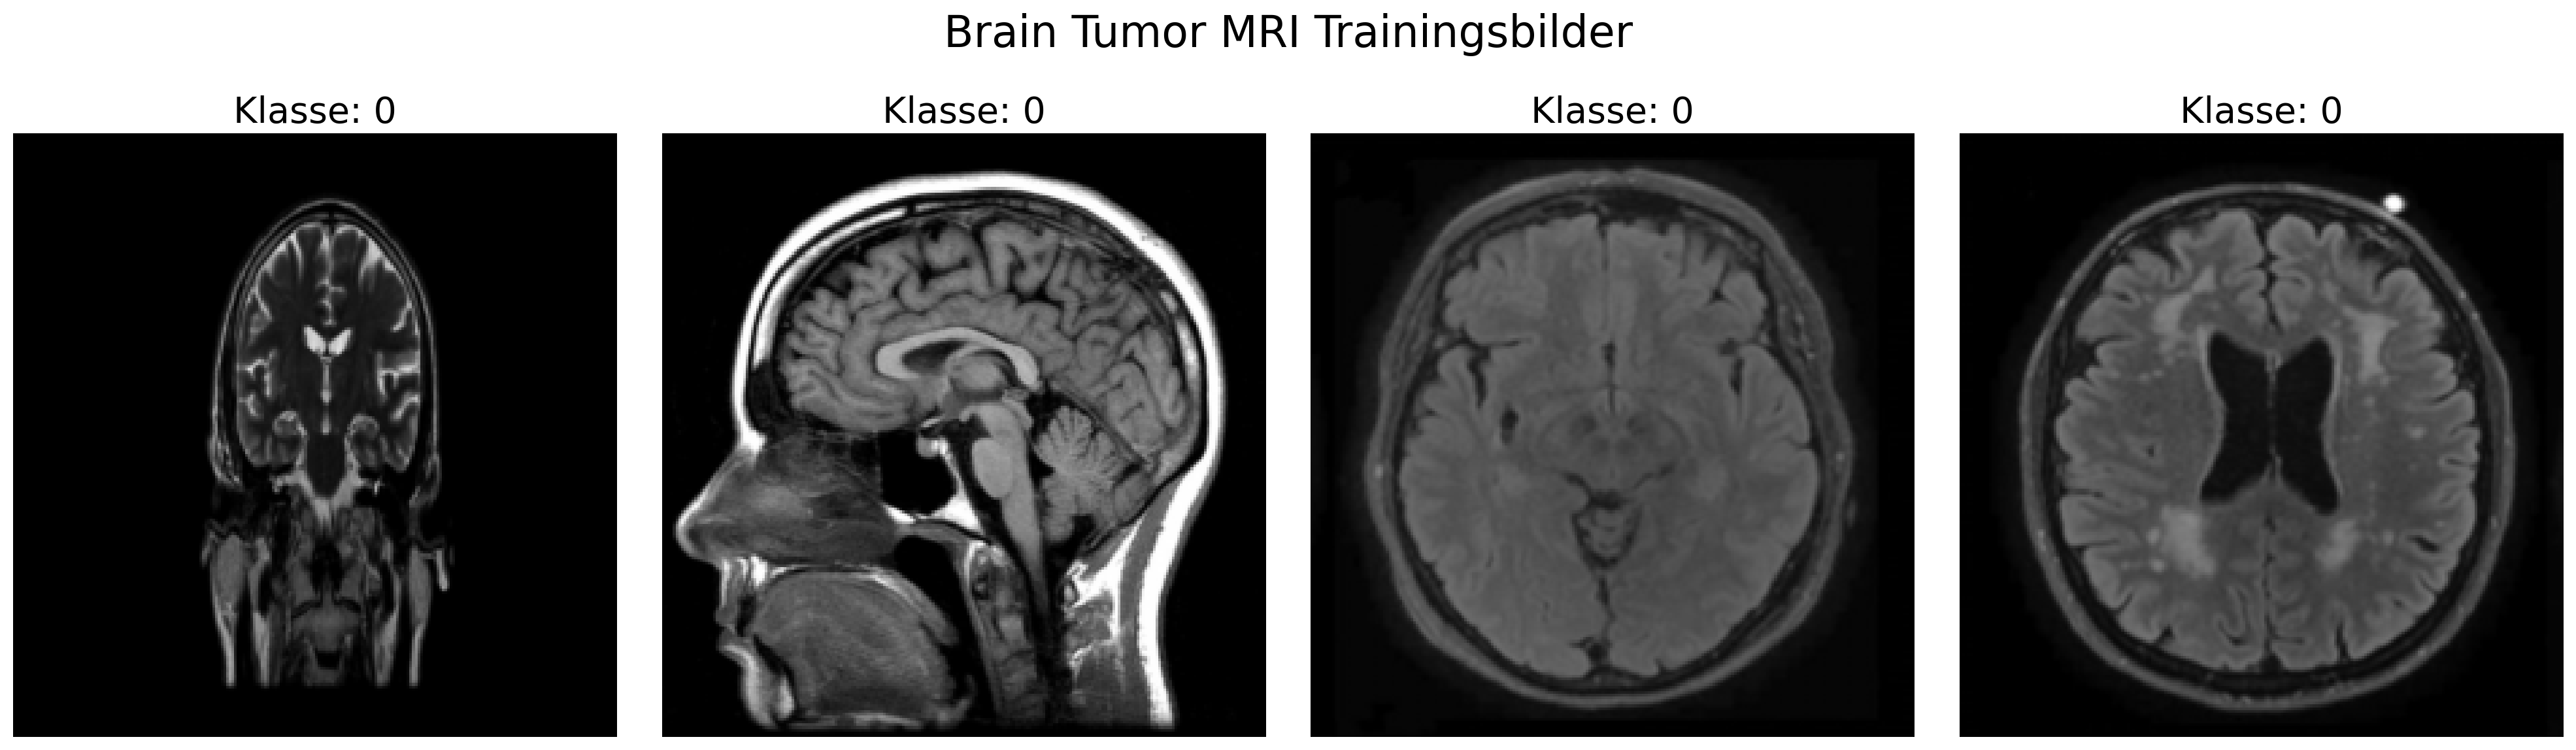
\includegraphics[width=\linewidth, height=4cm]{01-images/03-data/brain-klasse0.png}
    \caption{Beispiele von negativen Hirntumor Patienten vom Brain Tumor Datensatz}
    \label{fig:brain-klasse0}
\end{figure}

\begin{figure}[ht]
    \centering
    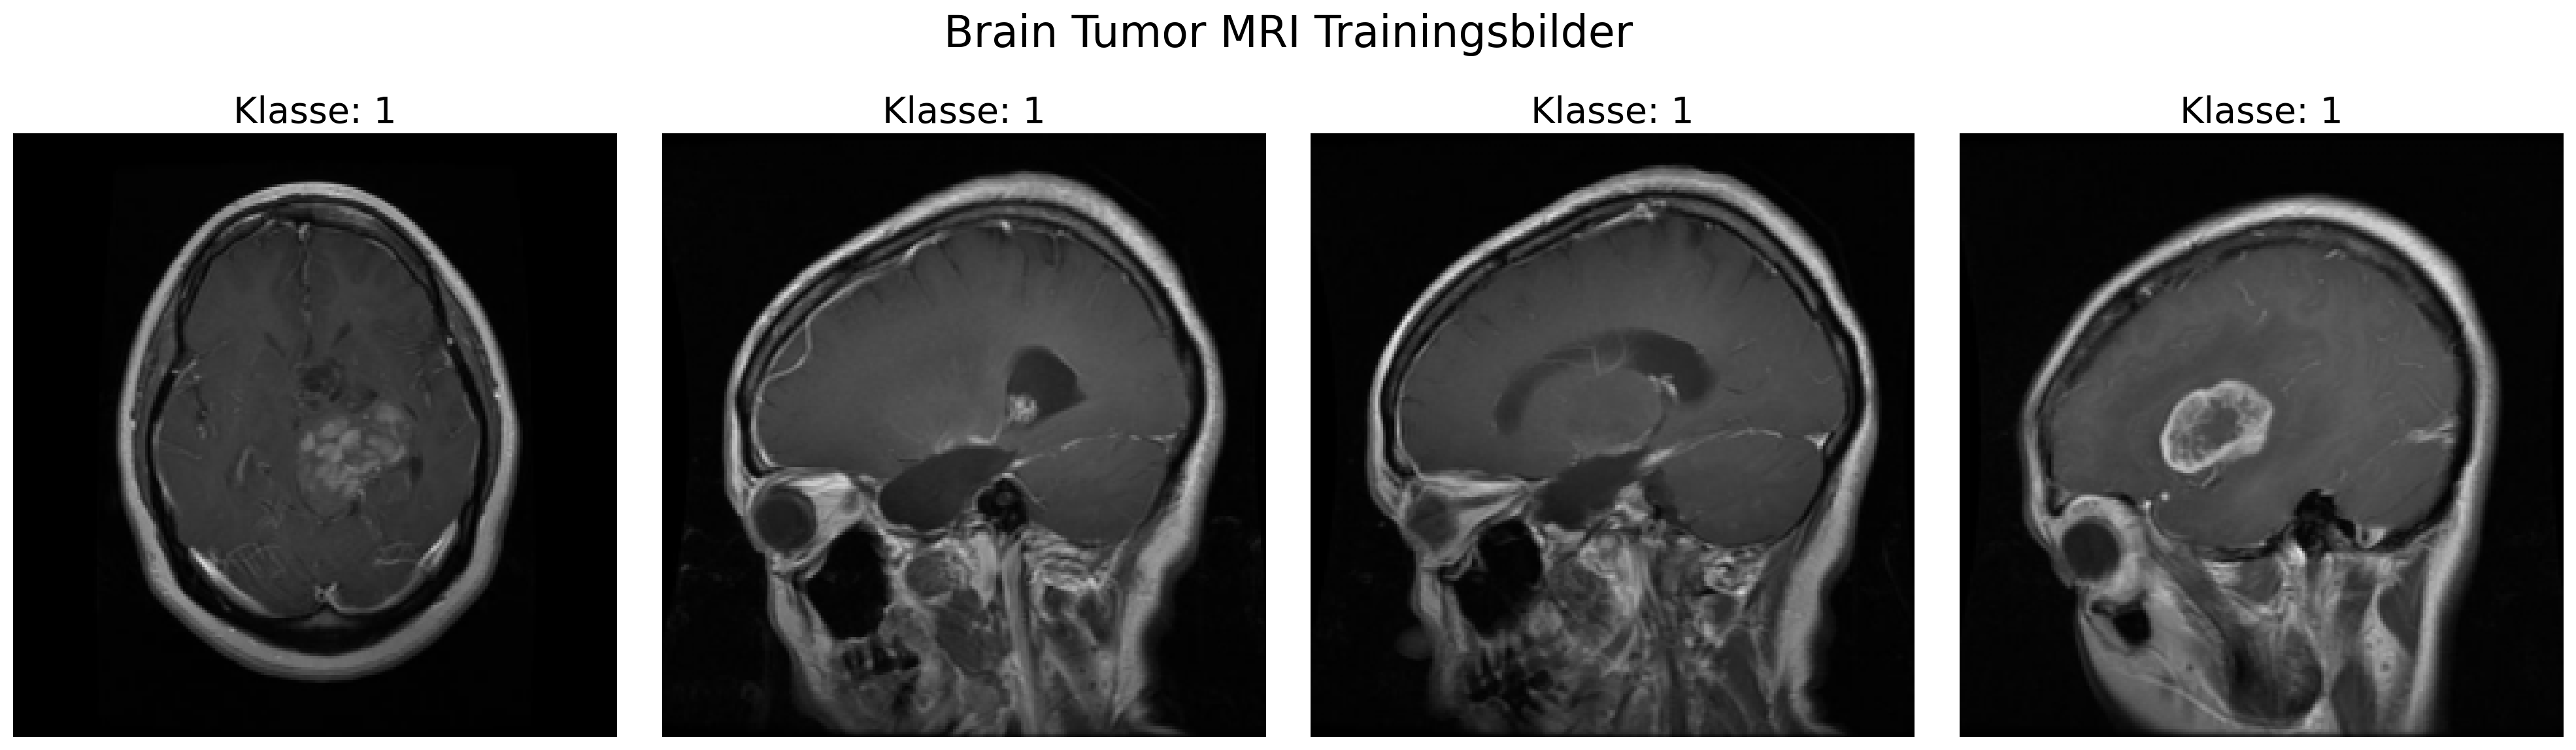
\includegraphics[width=\linewidth, height=4cm]{01-images/03-data/brain-klasse1.png}
    \caption{Beispiele von positiven Hirntumor Patienten vom Brain Tumor Datensatz}
    \label{fig:brain-klasse1}
\end{figure}

\newpage

\subsubsection{Hirntumorarten im Datensatz}
Im Datensatz für Hirntumoren gibt es vier Klassen. Drei davon sind positive Fälle, in denen Hirntumoren vorhanden sind. Eine Klasse ist negativ und beinhaltet keine Hirntumoren. Die drei positiven Klassen sind Gliome, Maligne Tumoren und Pituary.


\paragraph{Gliome}
Gliome sind eine Gruppe von Hirntumoren, die im Glia-Gewebe (Gewebe im Nervensystem) entstehen. Sie sind die häufigsten primären Hirntumoren bei Erwachsenen. Gliome werden nach ihren Ursprungszellen in Astrozytome, Oligodendrogliome und Ependymome unterteilt. Die Symptome variieren je nach Lage und Grösse des Tumors und können Kopfschmerzen, Anfälle und neurologische Defizite umfassen. Die Behandlung erfolgt in der Regel durch eine Kombination von Operation, Strahlentherapie und Chemotherapie.

\paragraph{Malignent}
Maligne Tumoren sind bösartige Wucherungen, die unkontrolliert wachsen und in umliegendes Gewebe eindringen können. Sie haben die Fähigkeit, Metastasen zu bilden, was bedeutet, dass sie sich auf andere Teile des Körpers ausbreiten können. Die Behandlung von malignen Tumoren umfasst in der Regel eine Kombination aus Operation, Strahlentherapie und Chemotherapie. Die Prognose hängt von der Art, dem Stadium und der Lage des Tumors ab.

\paragraph{Pituary}
Hypophysenadenome sind gutartige Tumoren der Hypophyse, einer kleinen Drüse im Gehirn, die wichtige Hormone produziert. Obwohl sie meist nicht bösartig sind, können sie aufgrund ihrer Lage und Hormonproduktion erhebliche gesundheitliche Probleme verursachen. Symptome können Kopfschmerzen, Sehstörungen und hormonelle Ungleichgewichte umfassen. Die Behandlung umfasst in der Regel eine Operation und, in einigen Fällen, medikamentöse Therapie oder Strahlentherapie.

\subsubsection{Datenpartitionierung} \label{chap:Brain-Tumor-Partition}

Der Datensatz enthält ursprünglich nur ein Trainings- und ein Testset. Da uns ein Validierungsset fehlt, erstellen wir dieses aus dem gegebenen Trainingsset. Der Datensatz umfasst vier Klassen, drei davon sind Tumorklassen und eine Klasse ist kein Tumor. Die Verteilung der Klassen ist in der Tabelle \ref{tab:mri-orginale-klassenverteilung} zu sehen. Ersichtlich ist, dass in dem Datensatz positive Tumorklassen deutlich mehr vertreten sind als keine Tumore. Da wir uns für unsere These auf die binäre Klassifikation stützen, fassen wir die drei Hirntumoren Klassen Pituitary, Glioma, Meningioma zu einem positiven Gehirn Tumor Klasse und kein Tumor als negative Klasse und erhalten somit die Tabelle \ref{tab:mri-binaere-klassenverteilung}.

\begin{table}[ht]
\centering
\begin{tabular}{@{}ccccc@{}}
\toprule
 Partition & \multicolumn{4}{c}{Klassenverteilung}        \\ 
\cmidrule(l){2-5}
           & Pituitary & Glioma & Meningioma & kein Tumor \\ 
\midrule 
Train      & 662 & 661 & 658 & 317 \\
Validation & 165 & 165 & 164 & 78  \\
Test       & 74  & 100 & 115 & 105 \\ 
\bottomrule
\end{tabular}
\caption{Ursprüngliche Klassenaufteilung von Hirntumoren}
\label{tab:mri-orginale-klassenverteilung}
\end{table}

Die Verteilungsverhältnisse waren ursprünglich 70.4\% Trainings- und 29.6\% Testbilder. Da ein analoger Datensatz, wie beim COVIDx, einfacher zu handhaben ist, haben wir den ursprünglichen Testdatensatz weiter unterteilt, und zwar in 17.5\% Validierungs- und 12.1\% Testdaten. Bevor wir die positiven Klassen zusammengefasst haben, herrschte eine Klassenimbalance, die wir bei der Partitionierung in Train-, Validierung, und Testset mitberücksichtigt haben. Die Tabelle \ref{tab:mri-binaere-klassenverteilung} zeigt die Anzahl an Bilder in absolut, relativ und die Klassenverteilung von positive, negative Tumorbilder für jede Datenpartition auf.

\begin{table}[ht]
\centering
\begin{tabular}{@{}cccccc@{}}
\toprule
Partition & \multicolumn{2}{c}{Anzahl Bilder} & \multicolumn{2}{c}{Klassenverteilung} & Positiv-Verhältnis\\ 
\cmidrule(lr){2-3} \cmidrule(lr){4-5} 
           & Absolut & Relativ & Positiv & Negativ \\ 
\midrule
Train      & 2298 & 0.704 & 1981 & 317 & 0.862 \\
Validation & 572  & 0.175 & 494  & 78  & 0.864 \\
Test       & 394  & 0.121 & 289  & 105 & 0.736 \\ 
\bottomrule
\end{tabular}
\caption{Binäre Klassenverteilung von Hirntumoren}
\label{tab:mri-binaere-klassenverteilung}
\end{table}

\subsubsection{Datenexploration}

Die Histogramme der Hirntumor-Klassifikation sehen im Vergleich zum COVIDx CXR-4-Datensatz deutlich unterschiedlich aus. So ist klar in den Beispielen ersichtlich, dass die Intensität von niedrigeren Pixelwerten sehr hoch.

\begin{figure}[ht]
    \centering
    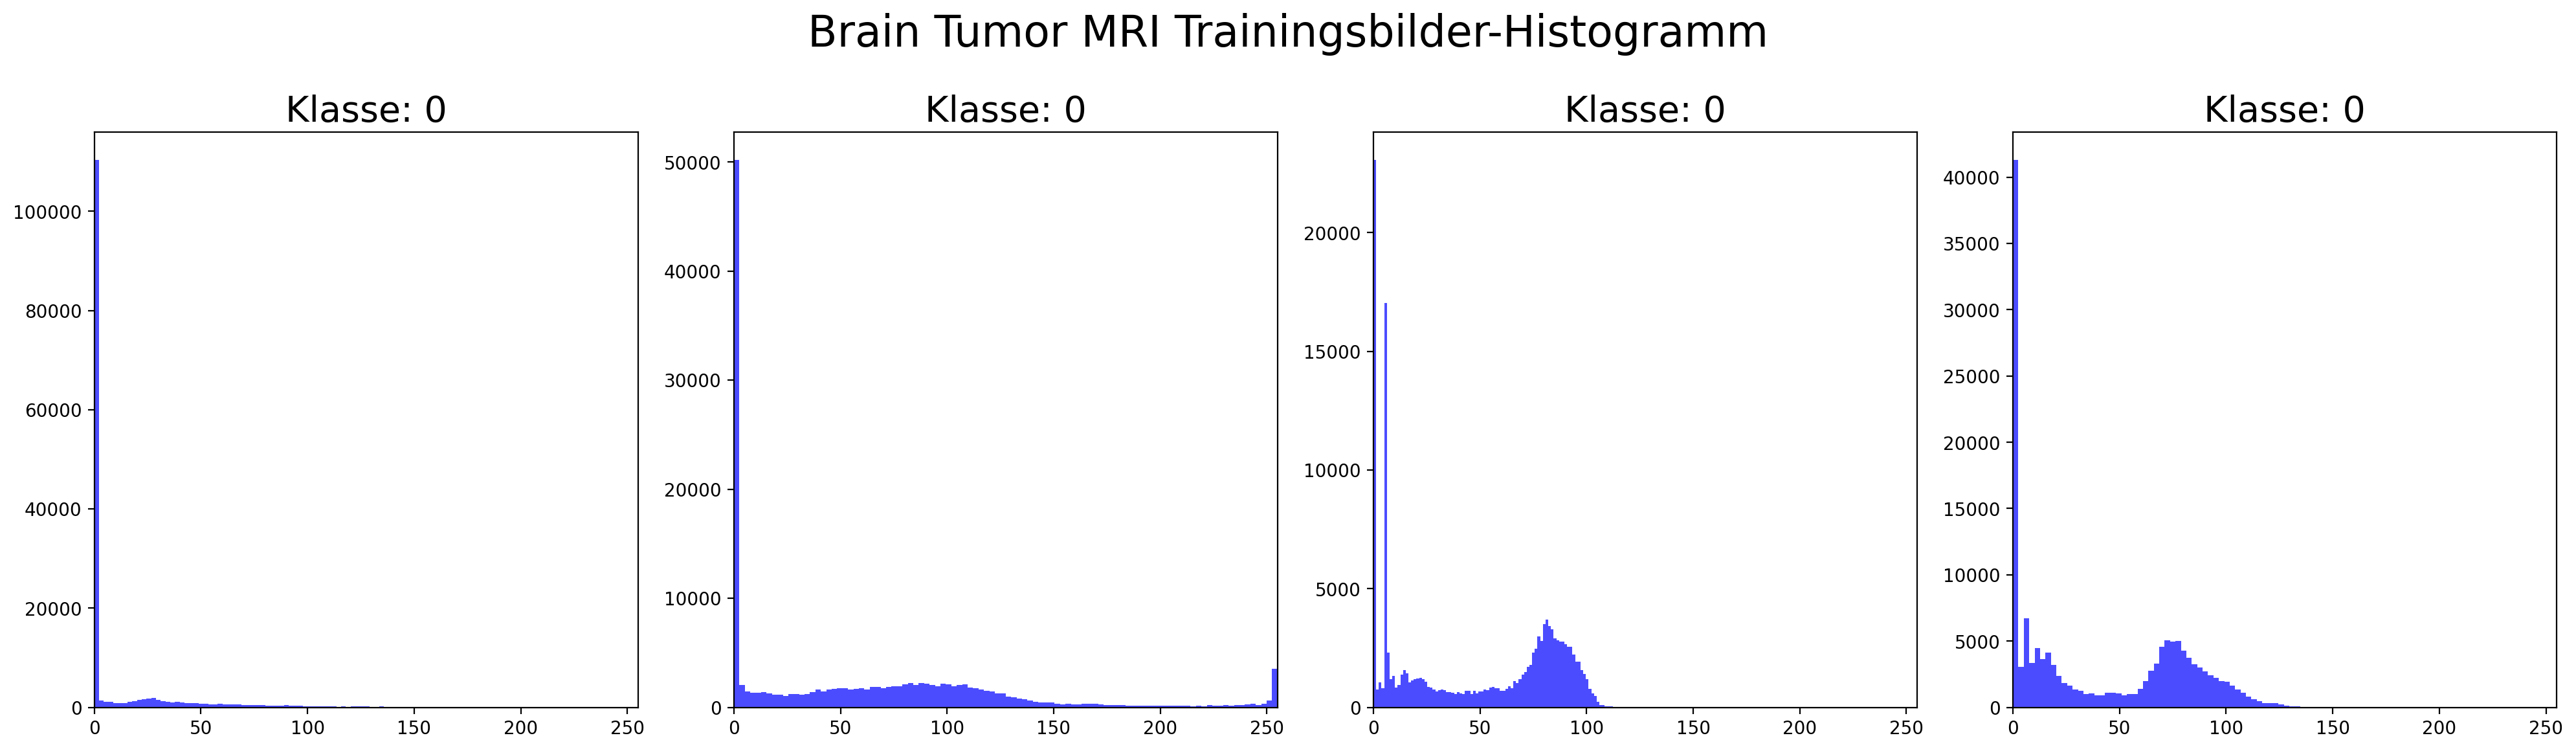
\includegraphics[width=\linewidth, height=4cm]{01-images/03-data/brain-klasse0-hist.png}
    \caption{Histogramm der Pixelverteilung von Abbildung \ref{fig:brain-klasse0}}
    \label{fig:brain-klasse0-hist}
\end{figure}

\begin{figure}[ht]
    \centering
    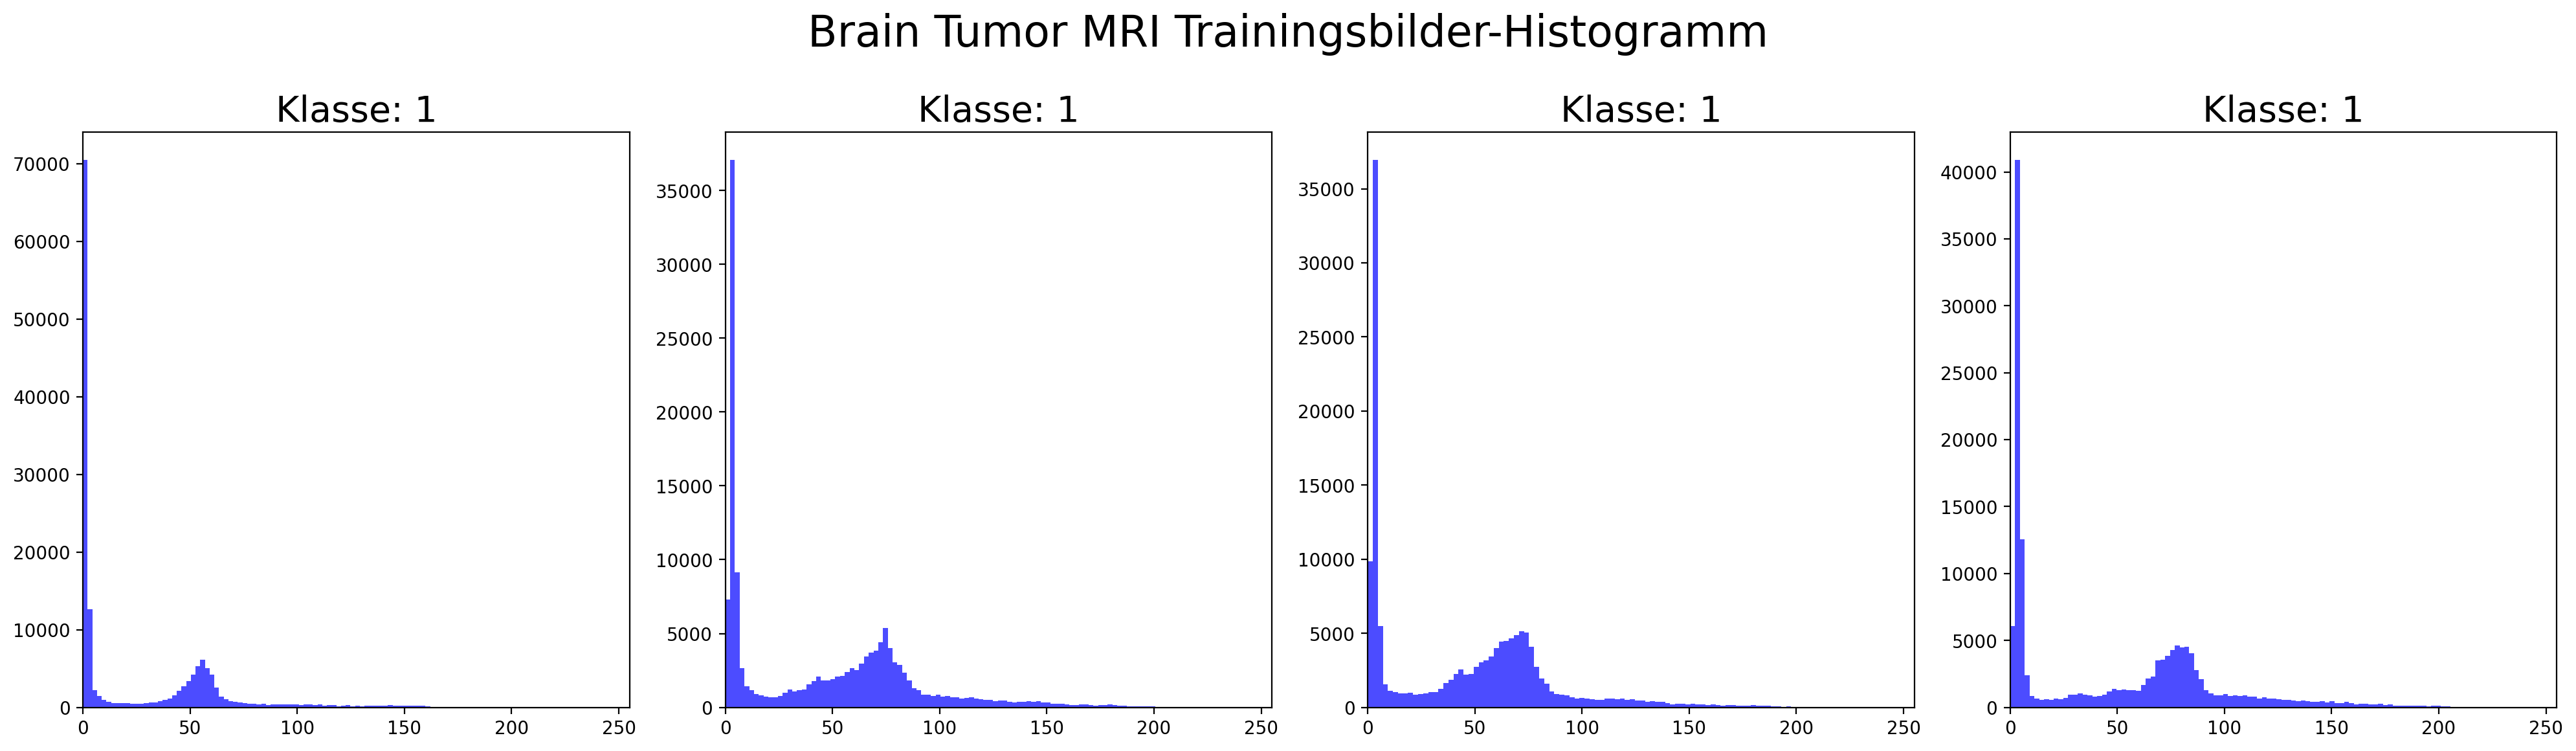
\includegraphics[width=\linewidth, height=4cm]{01-images/03-data/brain-klasse1-hist.png}
    \caption{Histogramm der Pixelverteilung von Abbildung \ref{fig:brain-klasse1}}
    \label{fig:brain-klasse1-hist}
\end{figure}

Die niedrigen Pixelwerte in einem Bild deuten darauf hin, dass viele dunkle Bereiche vorhanden sind. Es liegt nahe, dass dies der Hintergrund der MRI-Bilder ist und somit einen Grossteil der Informationen ausmacht, die keine relevanten Details enthalten.



\subsection{Datenverteilung \& Testperofmance} \label{chap:Datenverteilung-Testperformance-mri}

Wie im Kapitel \ref{chap:Datenverteilung-Testperformance-covidx} haben wir das Problem der Performance auf den Testmetriken ebenfalls auf den MRI Datensatz. 

\subsubsection{Pixelverteilung} \label{chap:Pixelverteilung-TestProblemEda1-mri}


Das Vorgehen, analog zu dem im Kapitel \ref{chap:Pixelverteilung-TestProblemEda1-covidx} beschriebenen, nutzen wir für unseren Hirntumor Datenpartitionen. In der Abbildung \ref{fig:hist-datapartition-brain} zeigt die Histogramme der Pixelwerte für jede Datenpartition.

\begin{figure}[ht]
    \centering
    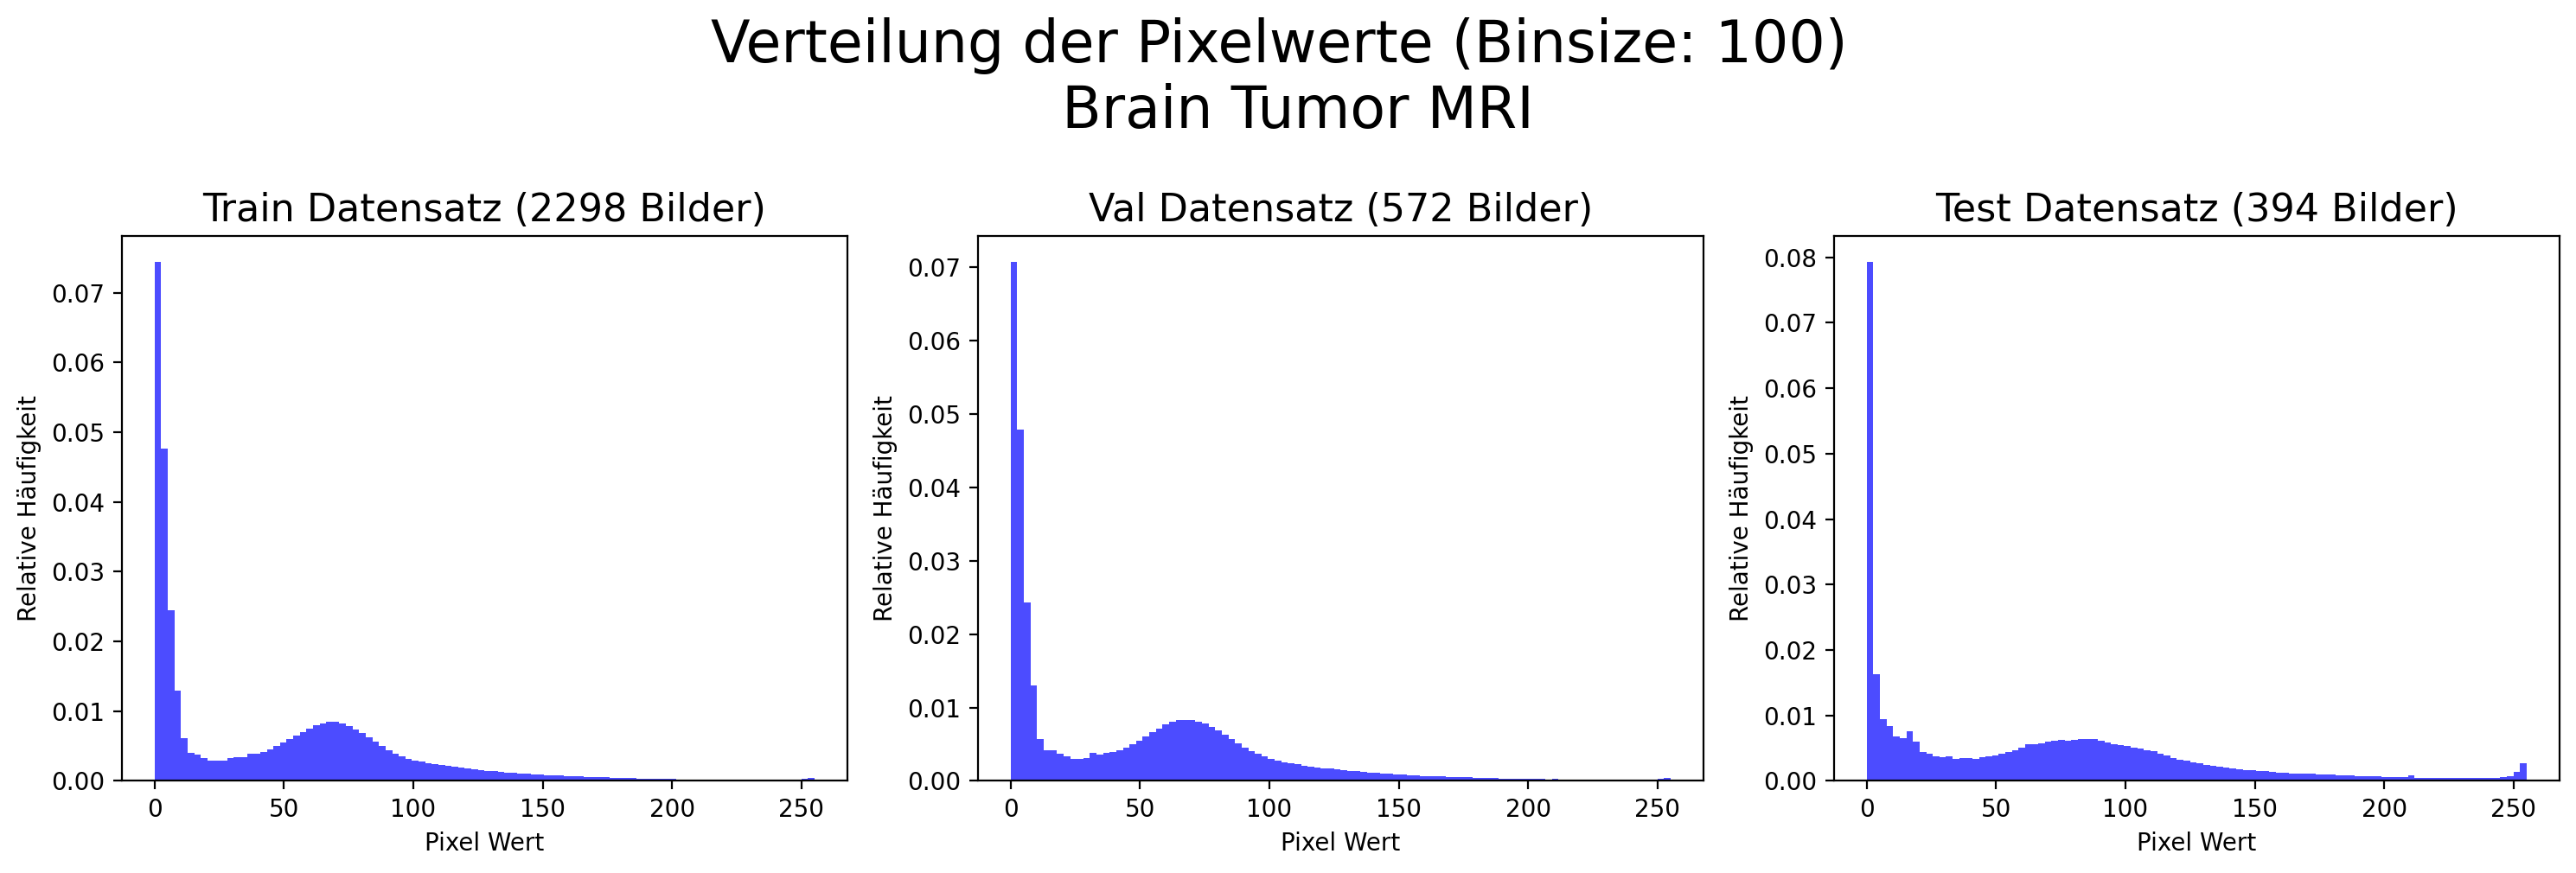
\includegraphics[width=\linewidth, height=5cm]{01-images/03-data/brain-Pixelverteilung-Partitionen.png}
    \caption{Histogramme der Pixelverteilung von Hirntumor in jeder Datenpartition}
    \label{fig:hist-datapartition-brain}
\end{figure}

Ein ähnliches Muster, das durch einen deutlichen Buckel gekennzeichnet ist, zeigt sich auch in diesem Hirntumor-Datensatz, jedoch mit einer Peakverschiebung. In den Hirntumor Histogrammen tritt dieser Peak typischerweise bei einem Pixelwert von etwa 80 auf. Sowohl die Trainings- als auch die Validierungspartition weisen ein vergleichbares Muster auf. In der Testpartition ist der Buckel allerdings weniger stark ausgeprägt. Zudem kommt es ab einem Pixelwert von 250 zu einem markanten Anstieg, der am Ende des Histogramms einen signifikanten Ausschlag verursacht. Eine mögliche Erklärung, dass die Testdatenpartition aus einer anderen Verteilung kommt. 

\subsubsection{Differenzbilder} \label{chap:Differenzenbilder-TestProblemEda2-mri}

Auch bei den Differenzbilder ist das Vorgehen, analog wie im Kapitel \ref{chap:Differenzenbilder-TestProblemEda2-covidx} beschrieben. 

\begin{figure}[ht]
    \centering
    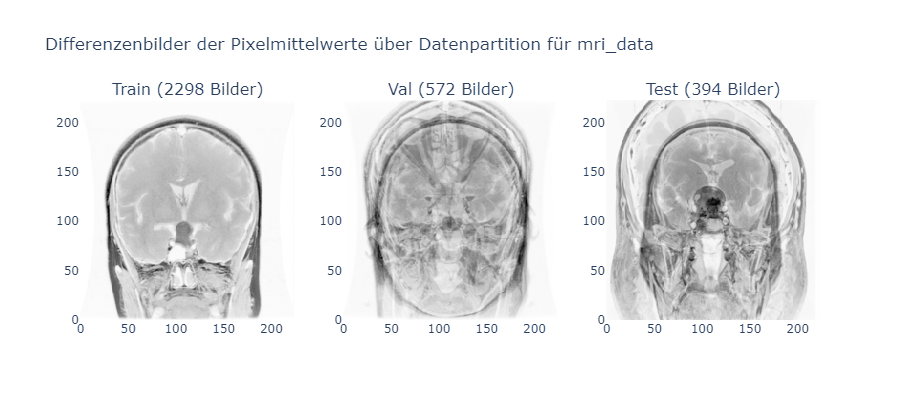
\includegraphics[width=\linewidth, height=5cm]{01-images/03-data/brain-Differenzenbilder-Partition.png}
    \caption{Differenzbilder von Hirntumor in jeder Datenpartition}
    \label{fig:differenzenbilder-datapartition-brain}
\end{figure}

In der Trainingspartition der Differenzbilder ist eine klare und detaillierte Konsistenz der Bilder vorhanden. In der Validierungs- und Testpartition ist dies jedoch nicht der Fall. Dort sind verschwommene Darstellungen zu erkennen, was auf die unterschiedliche Vielfalt der Bilder zurückzuführen ist. Dabei lässt sich visuell feststellen, dass die Verschwommenheit in der Validierungspartition nicht so stark ausgeprägt ist wie in der Testpartition.

\subsubsection{Feature Maps \& PCA} \label{chap:FeatureMaps-TestProblemEda3-mri}

\todo{Im Anhang hinzufuegen ? }

\newpage